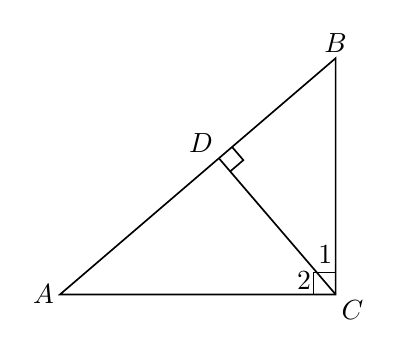
\begin{tikzpicture}[x=1cm,y=1cm,font=\normalsize,
 geometry edge/.style={solid,line width=.6pt},
 geometry mark/.style={solid,line width=.6pt},
 geometry label/.style={font=\normalsize,inner sep=2pt}]
\coordinate (A) at (-3.5,0);
\coordinate (B) at (0,3);
\coordinate (C) at (0,0);
\coordinate (D) at (-1.4824,1.7294);
\draw[geometry edge] (A)--(B)--(C)--cycle;
\draw[geometry edge] (C)--(D);
\draw[geometry mark] (C) ++(-0.28,0) -- ++(0,0.28) -- ++(0.28,0);
\draw[geometry mark] (D) ++(0.1671,0.1432) -- ++(0.1432,-0.1671) -- ++(-0.1671,-0.1432);
\node[geometry label,left] at (A) {$A$};
\node[geometry label,above] at (B) {$B$};
\node[geometry label,below right] at (C) {$C$};
\node[geometry label,above left] at (D) {$D$};
\node[font=\normalsize] at (-0.13,0.5) {$1$};
\node[font=\normalsize] at (-0.4,0.18) {$2$};
\end{tikzpicture}
